\documentclass{article}
\usepackage[utf8]{inputenc}
\usepackage[norsk]{babel}
\usepackage{mathtools} 
\usepackage{hyperref}
\usepackage{listings} 
\usepackage{graphicx}
\begin{document}
\begin{titlepage}
\begin{center}

\vspace*{3cm}
\textsc{\Huge D2b}\\[0.7cm]
\textsc{\medium TTM4100 - Communication Services and Networks}\\[0.3cm]
\textsc{\medium TDT4140 - Software Enigneering}\\[0.3cm]
\textsc{\medium TDT4145 - Data Modeling, Databases and Database Management Systems}\\[0.3cm]
\textsc{\medium TDT4180 - Human-Computer Interaction}\\[0.3cm]

\textbf{\Large Gruppe 7:} \\[0.2cm]
\text{\Large Espen Albert, Finn Inderhaug, Kristoffer Andreas Dalby} \\
\text{\Large Christoffer B. Nysæter, Andreas Wien, Jonas André Dalseth}\\[1cm]

\today

\end{center}
\end{titlepage}



\section{Description of the prototype}
% remember to put graphs har, use \begin{figure } from wiki
\begin{figure}[h!] 
    \begin{center} 
        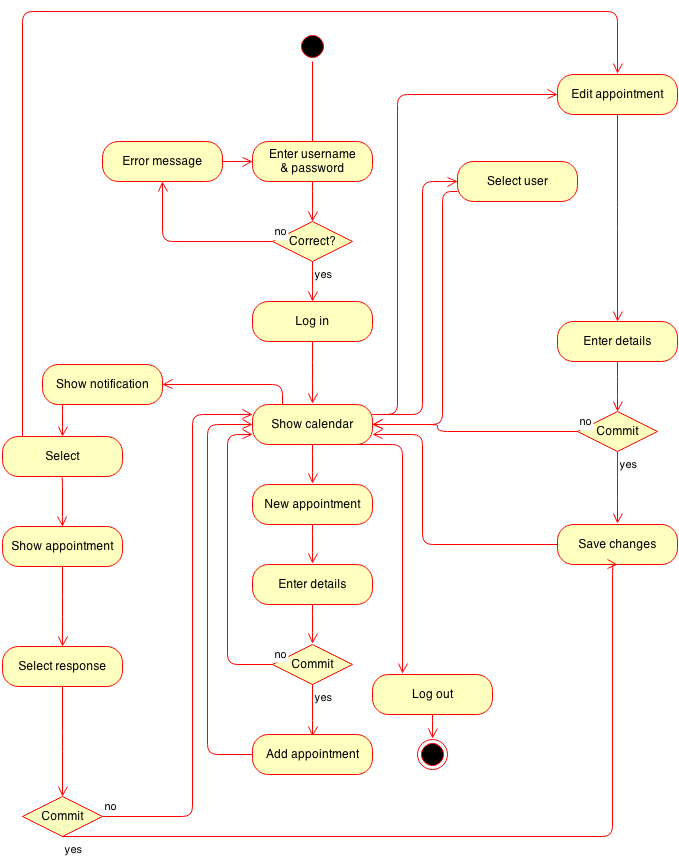
\includegraphics[width=8cm]{img/calendarStateDiagram.png}
        \caption{Calendar state diagram}
    \label{calendarstatediagram}
    \end{center}
\end{figure}

\newpage

\begin{figure}[h!] 
    \begin{center} 
        \includegraphics[width=8cm]{img/IMG_5600.png}
        \caption{Log in screen}
    \label{login}
    \end{center}
\end{figure}

Enter username and password in their respective JTextFields. Press the "Log in"-button to log in.

\begin{figure}[h!] 
    \begin{center} 
        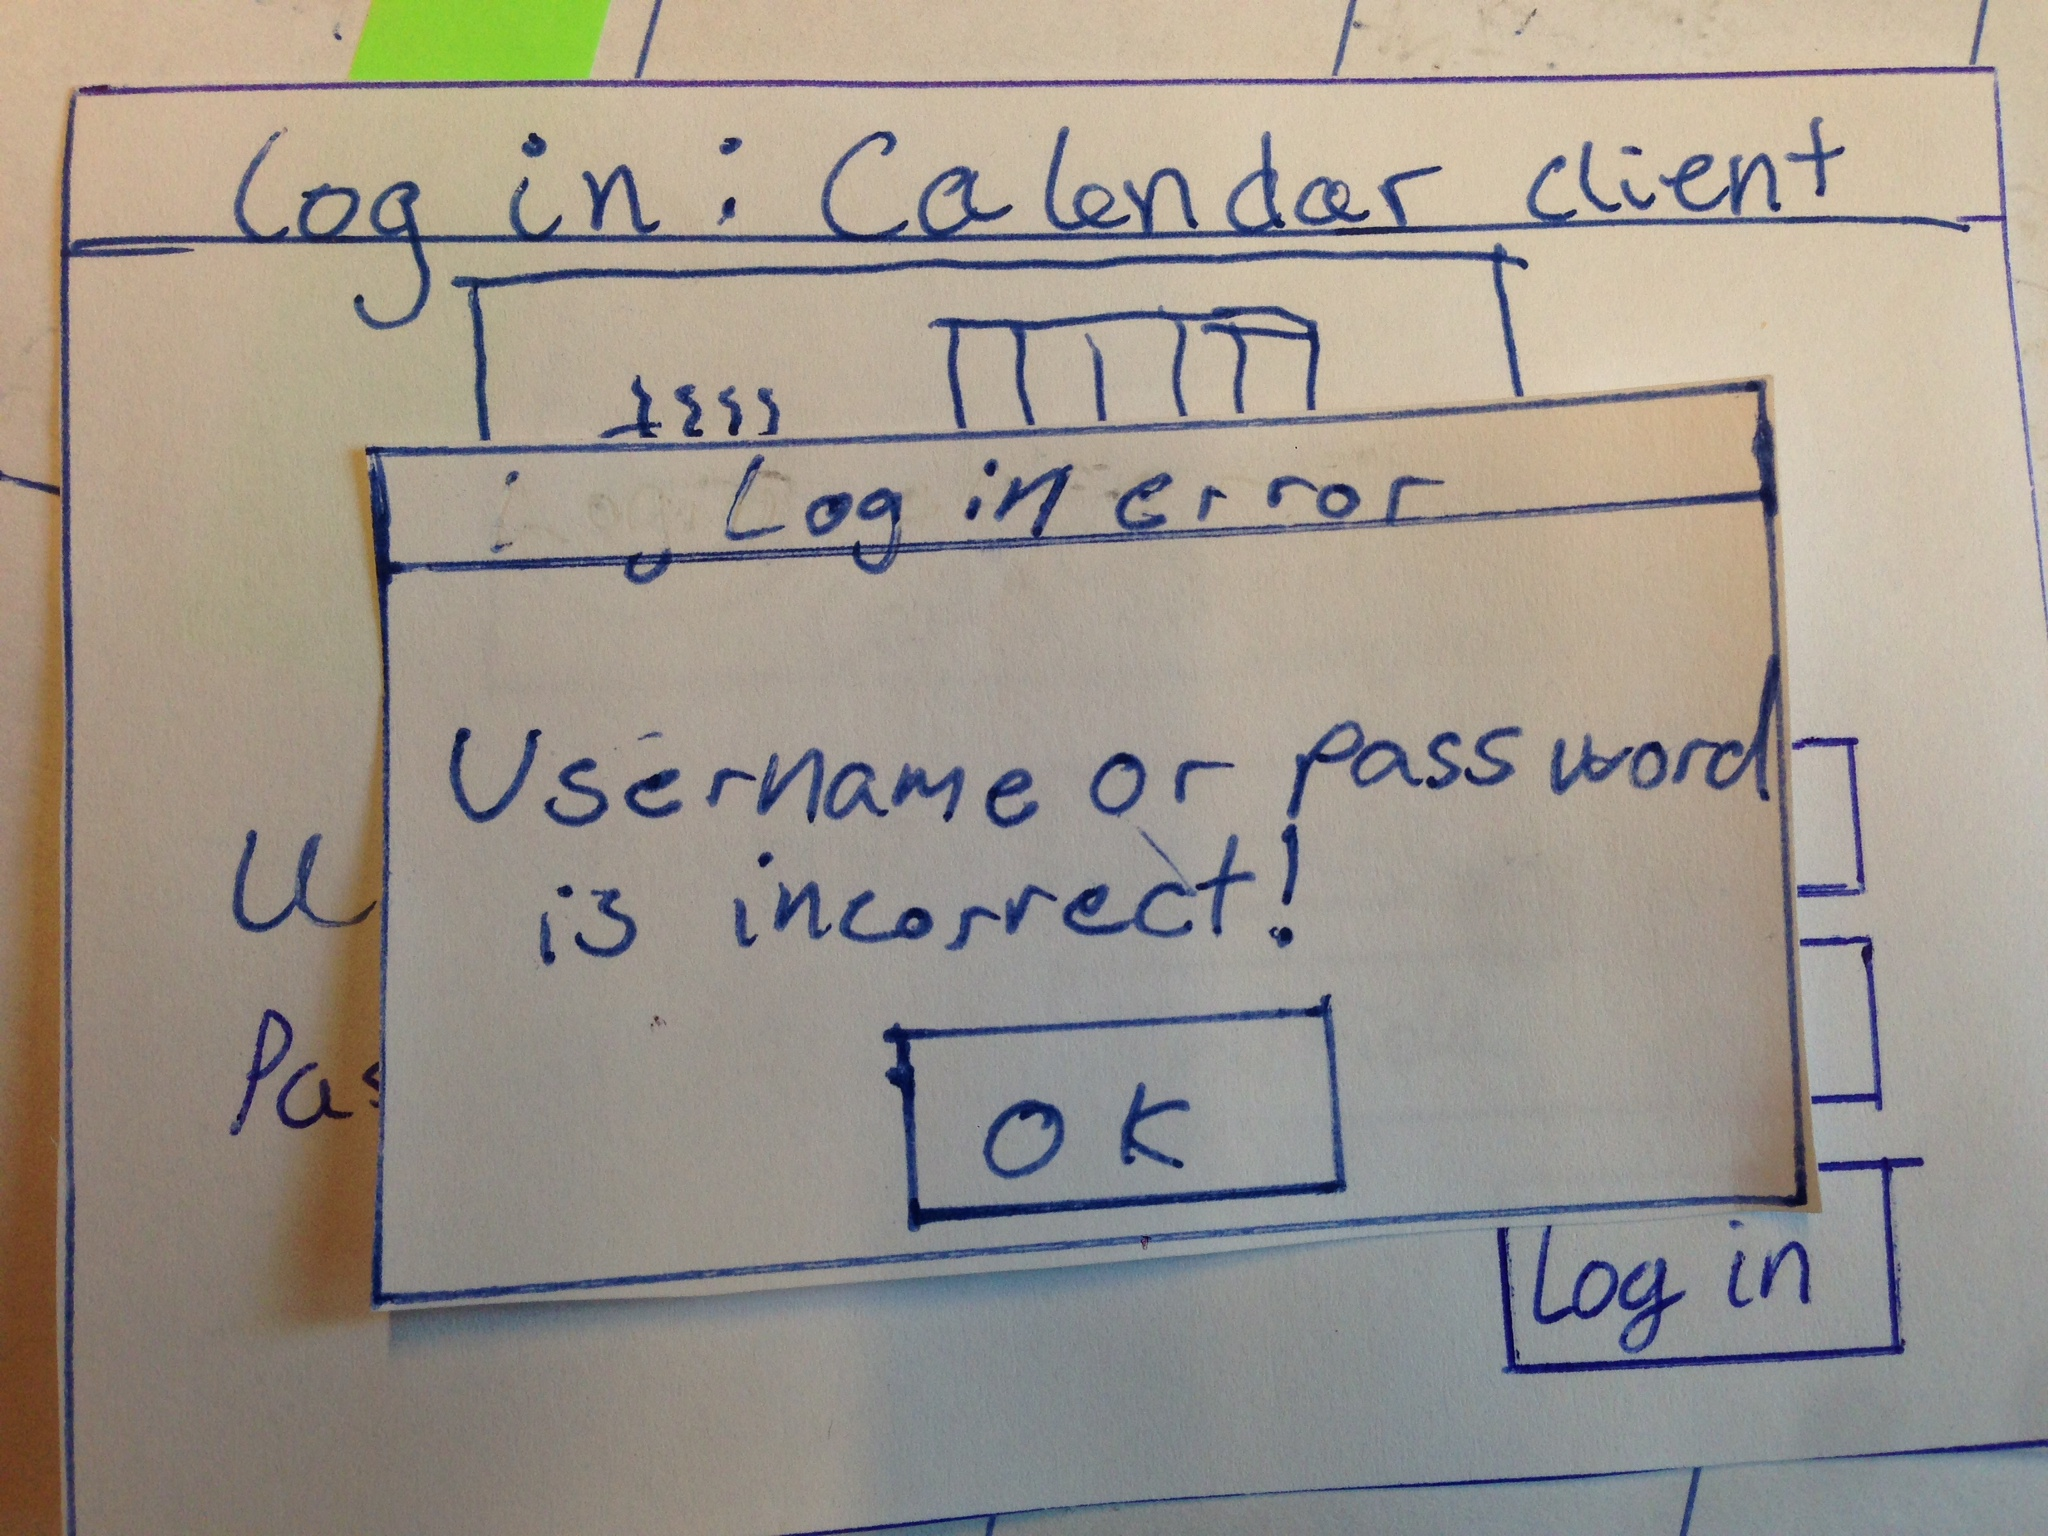
\includegraphics[width=8cm]{img/IMG_5612.JPG}
        \caption{Log in error}
    \label{loginerror}
    \end{center}
\end{figure}

If username or password is incorrect, this screen will show up. Press "OK"-button to close error message.

\newpage

\begin{figure}[h!] 
    \begin{center} 
        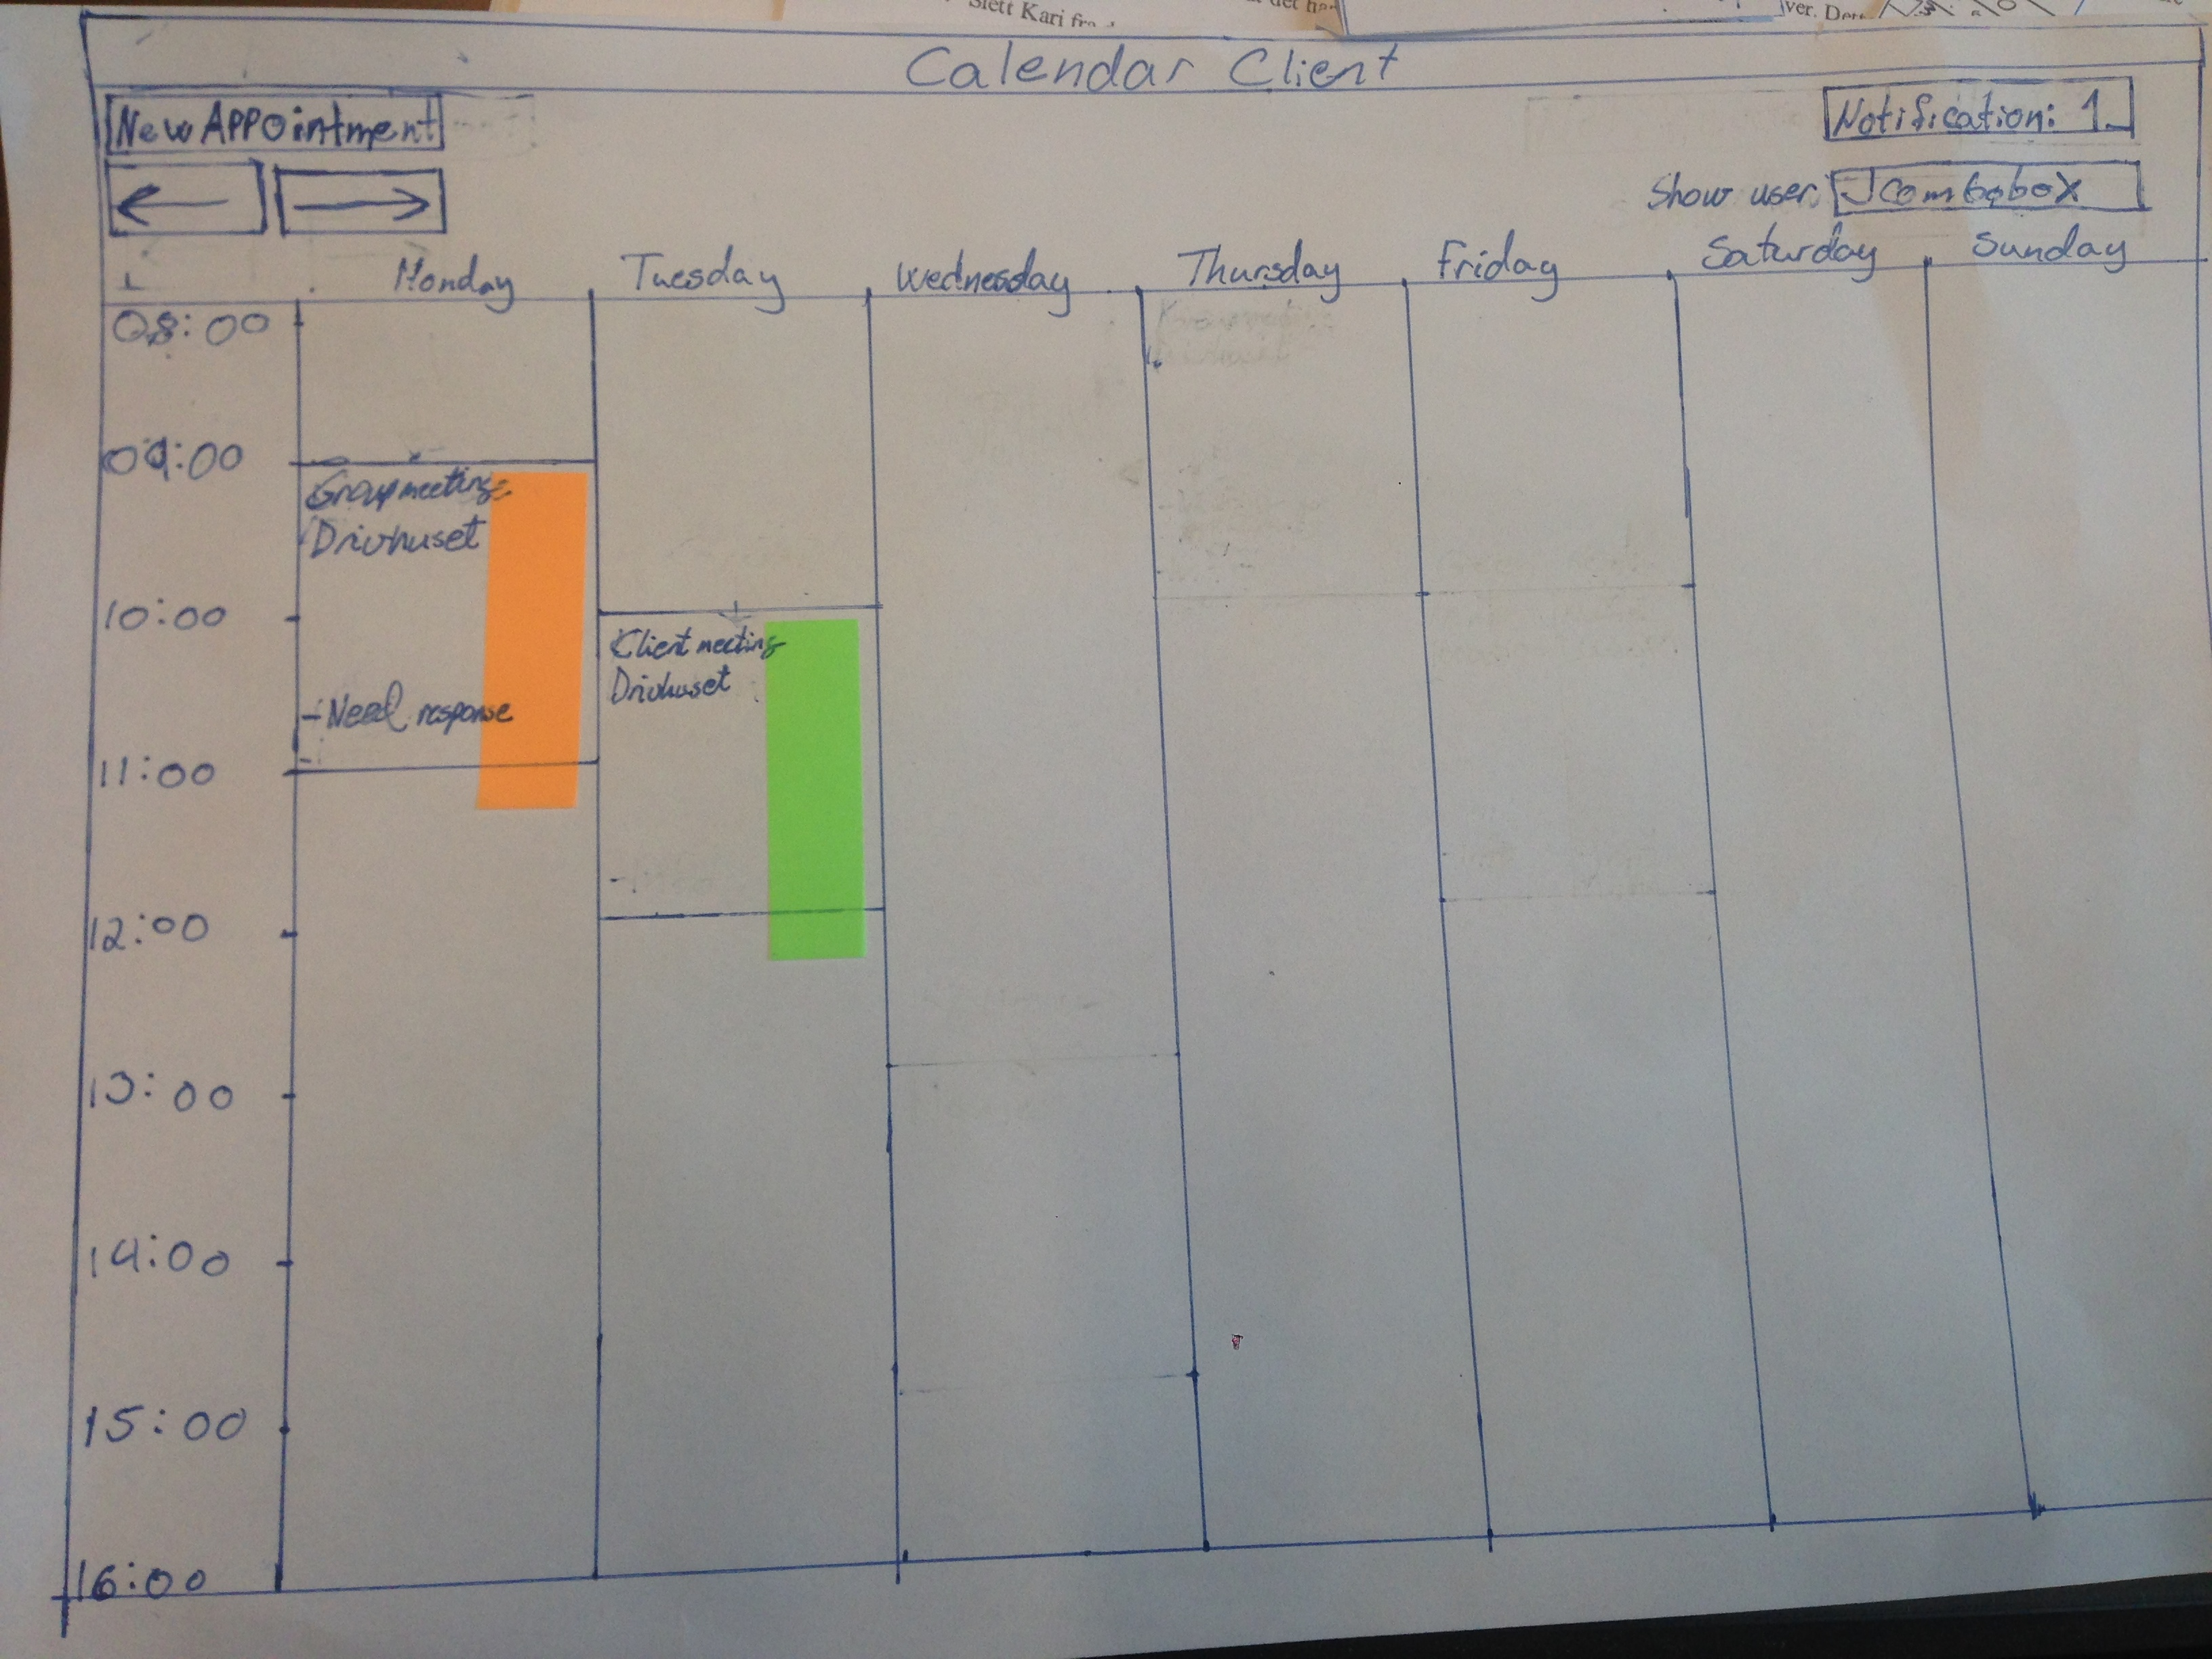
\includegraphics[width=8cm]{img/IMG_5601.JPG}
        \caption{Main view}
    \label{mainview}
    \end{center}
\end{figure}

The main view. From here it's possible to click "new appointment"-button to make a new appointment. When pressing the arrowbuttons, the next week or previous week will be shown. By clicking an appointment in the calendar, it's possible to edit or view the appointment. From the show user JComboBox, you can view other users calendar. By clicking the "notification"-button, you can check your notifications.

\begin{figure}[h!] 
    \begin{center} 
        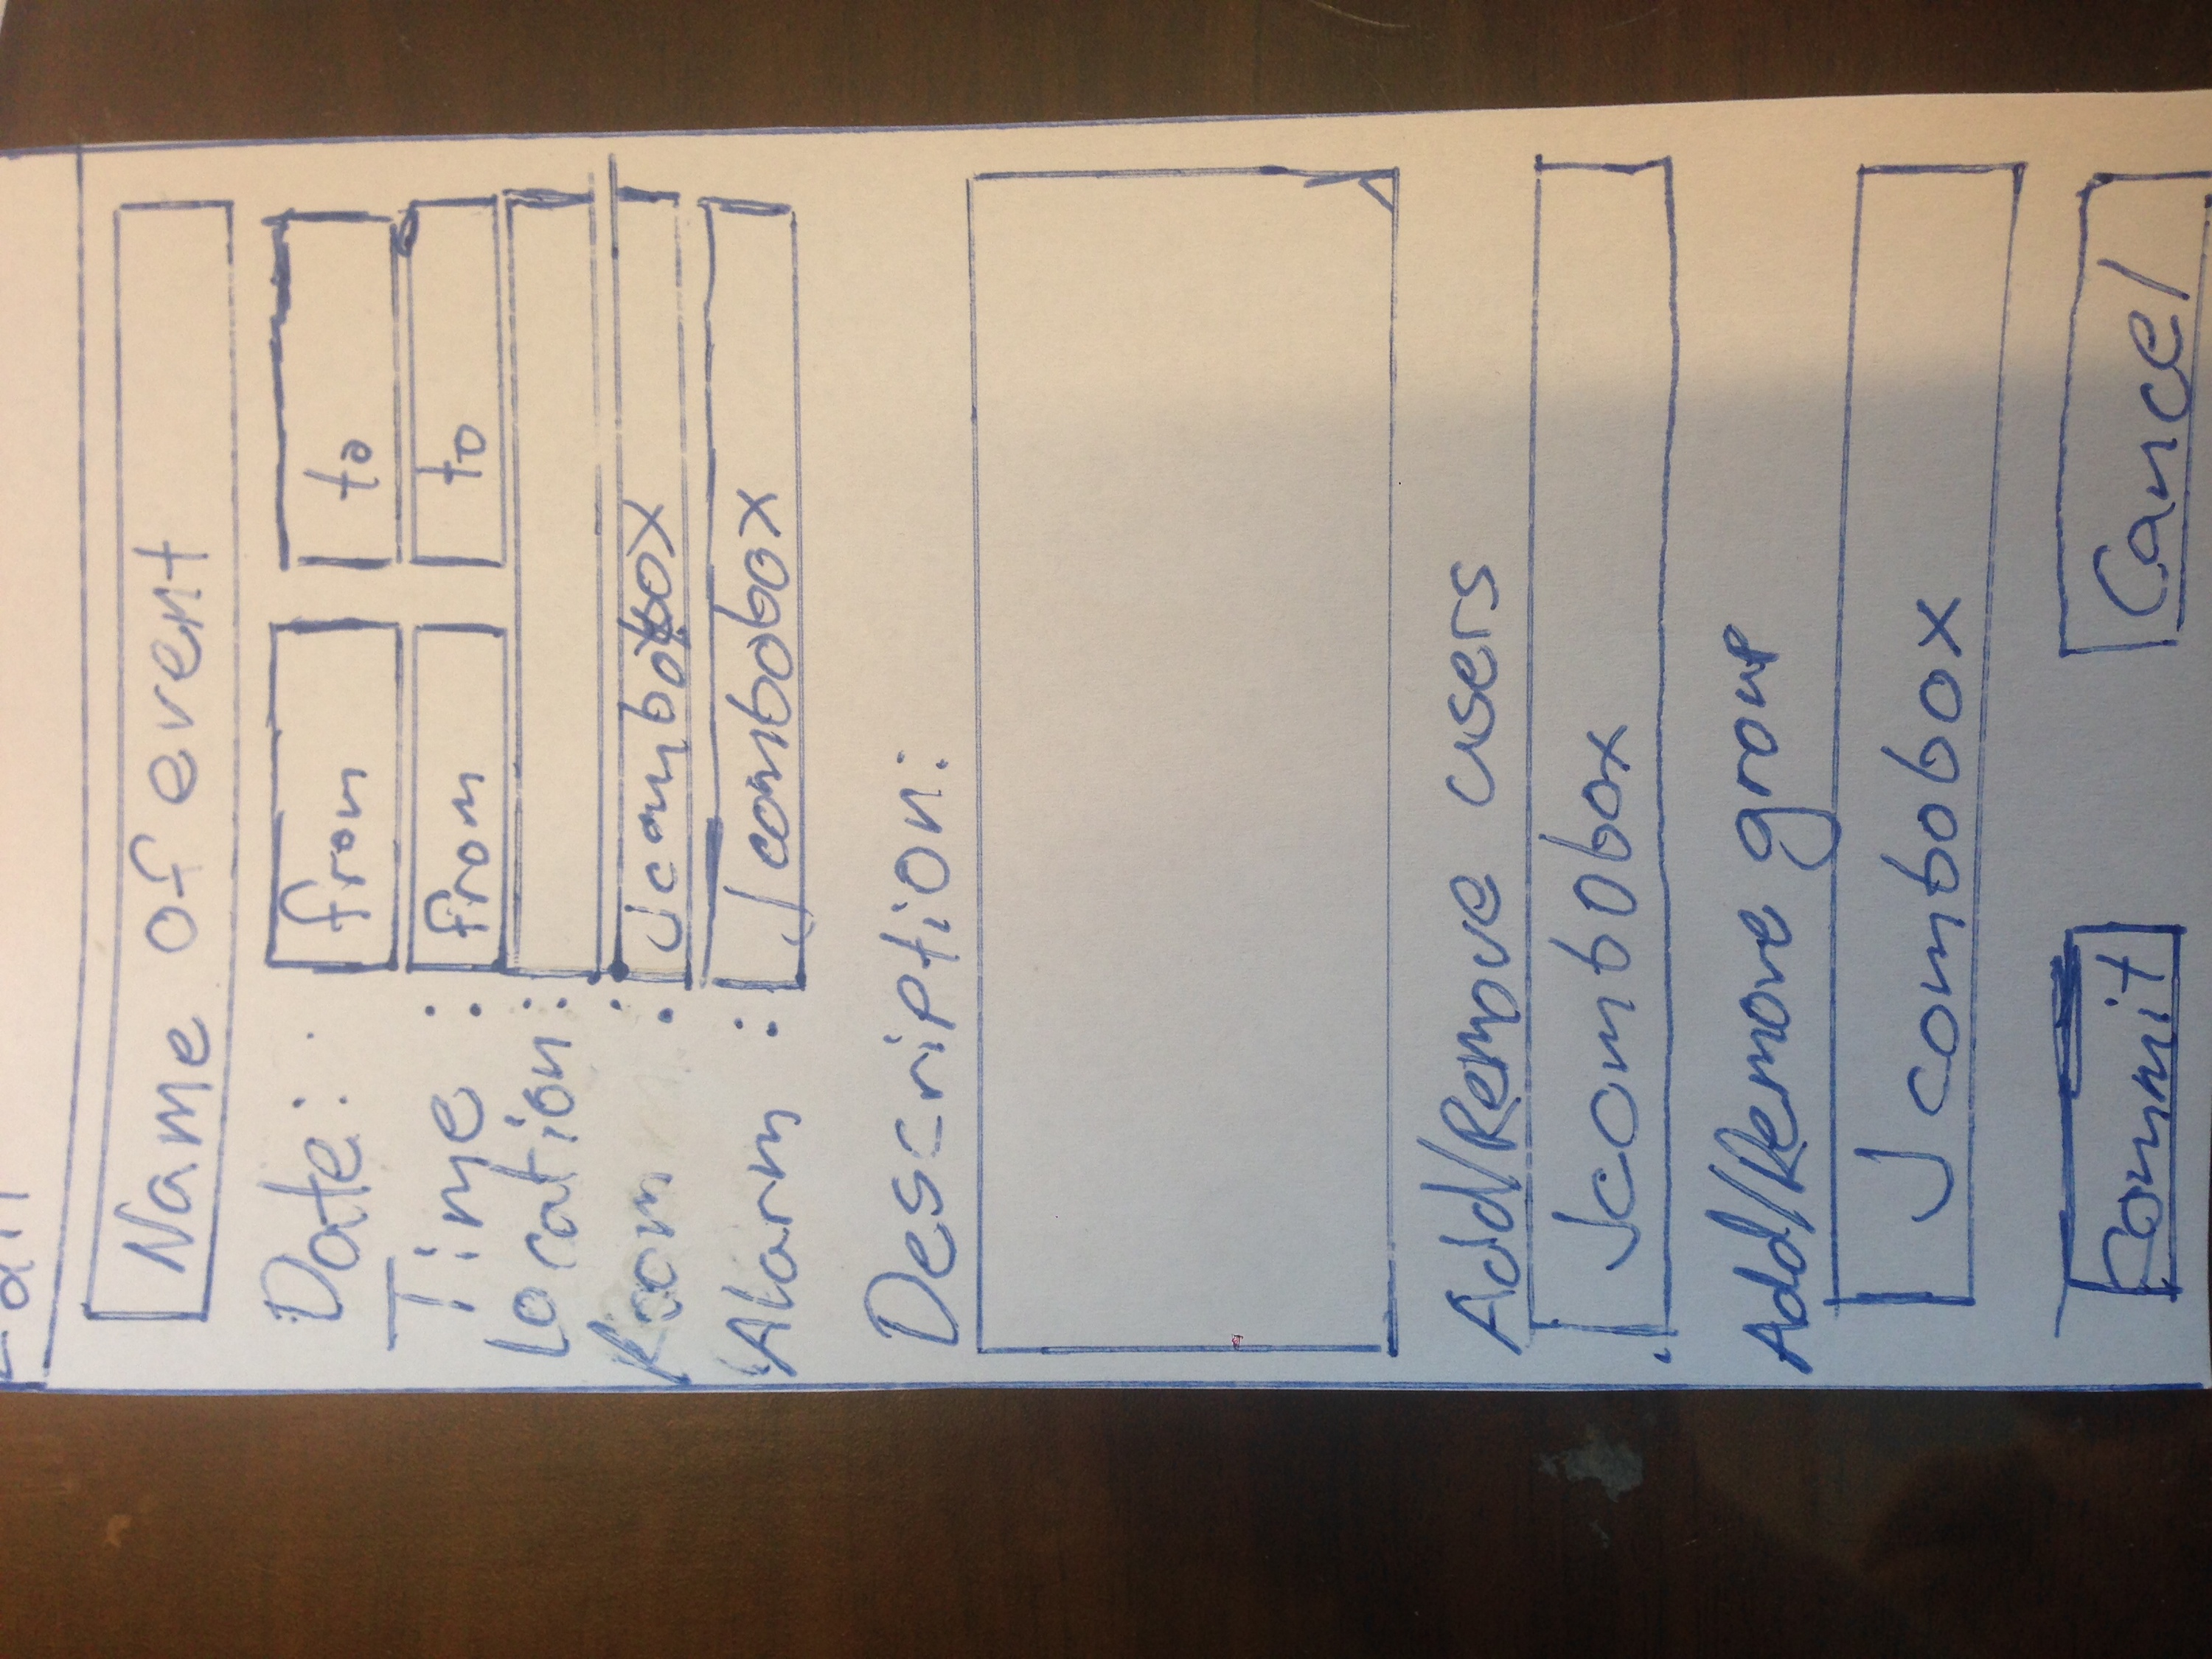
\includegraphics[width=8cm]{img/IMG_5602.png}
        \caption{Edit screen}
    \label{edit}
    \end{center}
\end{figure}

From this editscreen it's possible to enter time, date, room and alarm from dropdown-menus. Location and description are textfields that may be filled with text. In addition it's possible to add users and groups, through dropdown-menus.

\newpage

\begin{figure}[h!] 
    \begin{center} 
        \includegraphics[width=8cm]{img/IMG_5604.png}
        \caption{Room dropdown menu}
    \label{roomdropdown}
    \end{center}
\end{figure}

This is an example of a dropdownmenu.

\newpage

\begin{figure}[h!] 
    \begin{center} 
        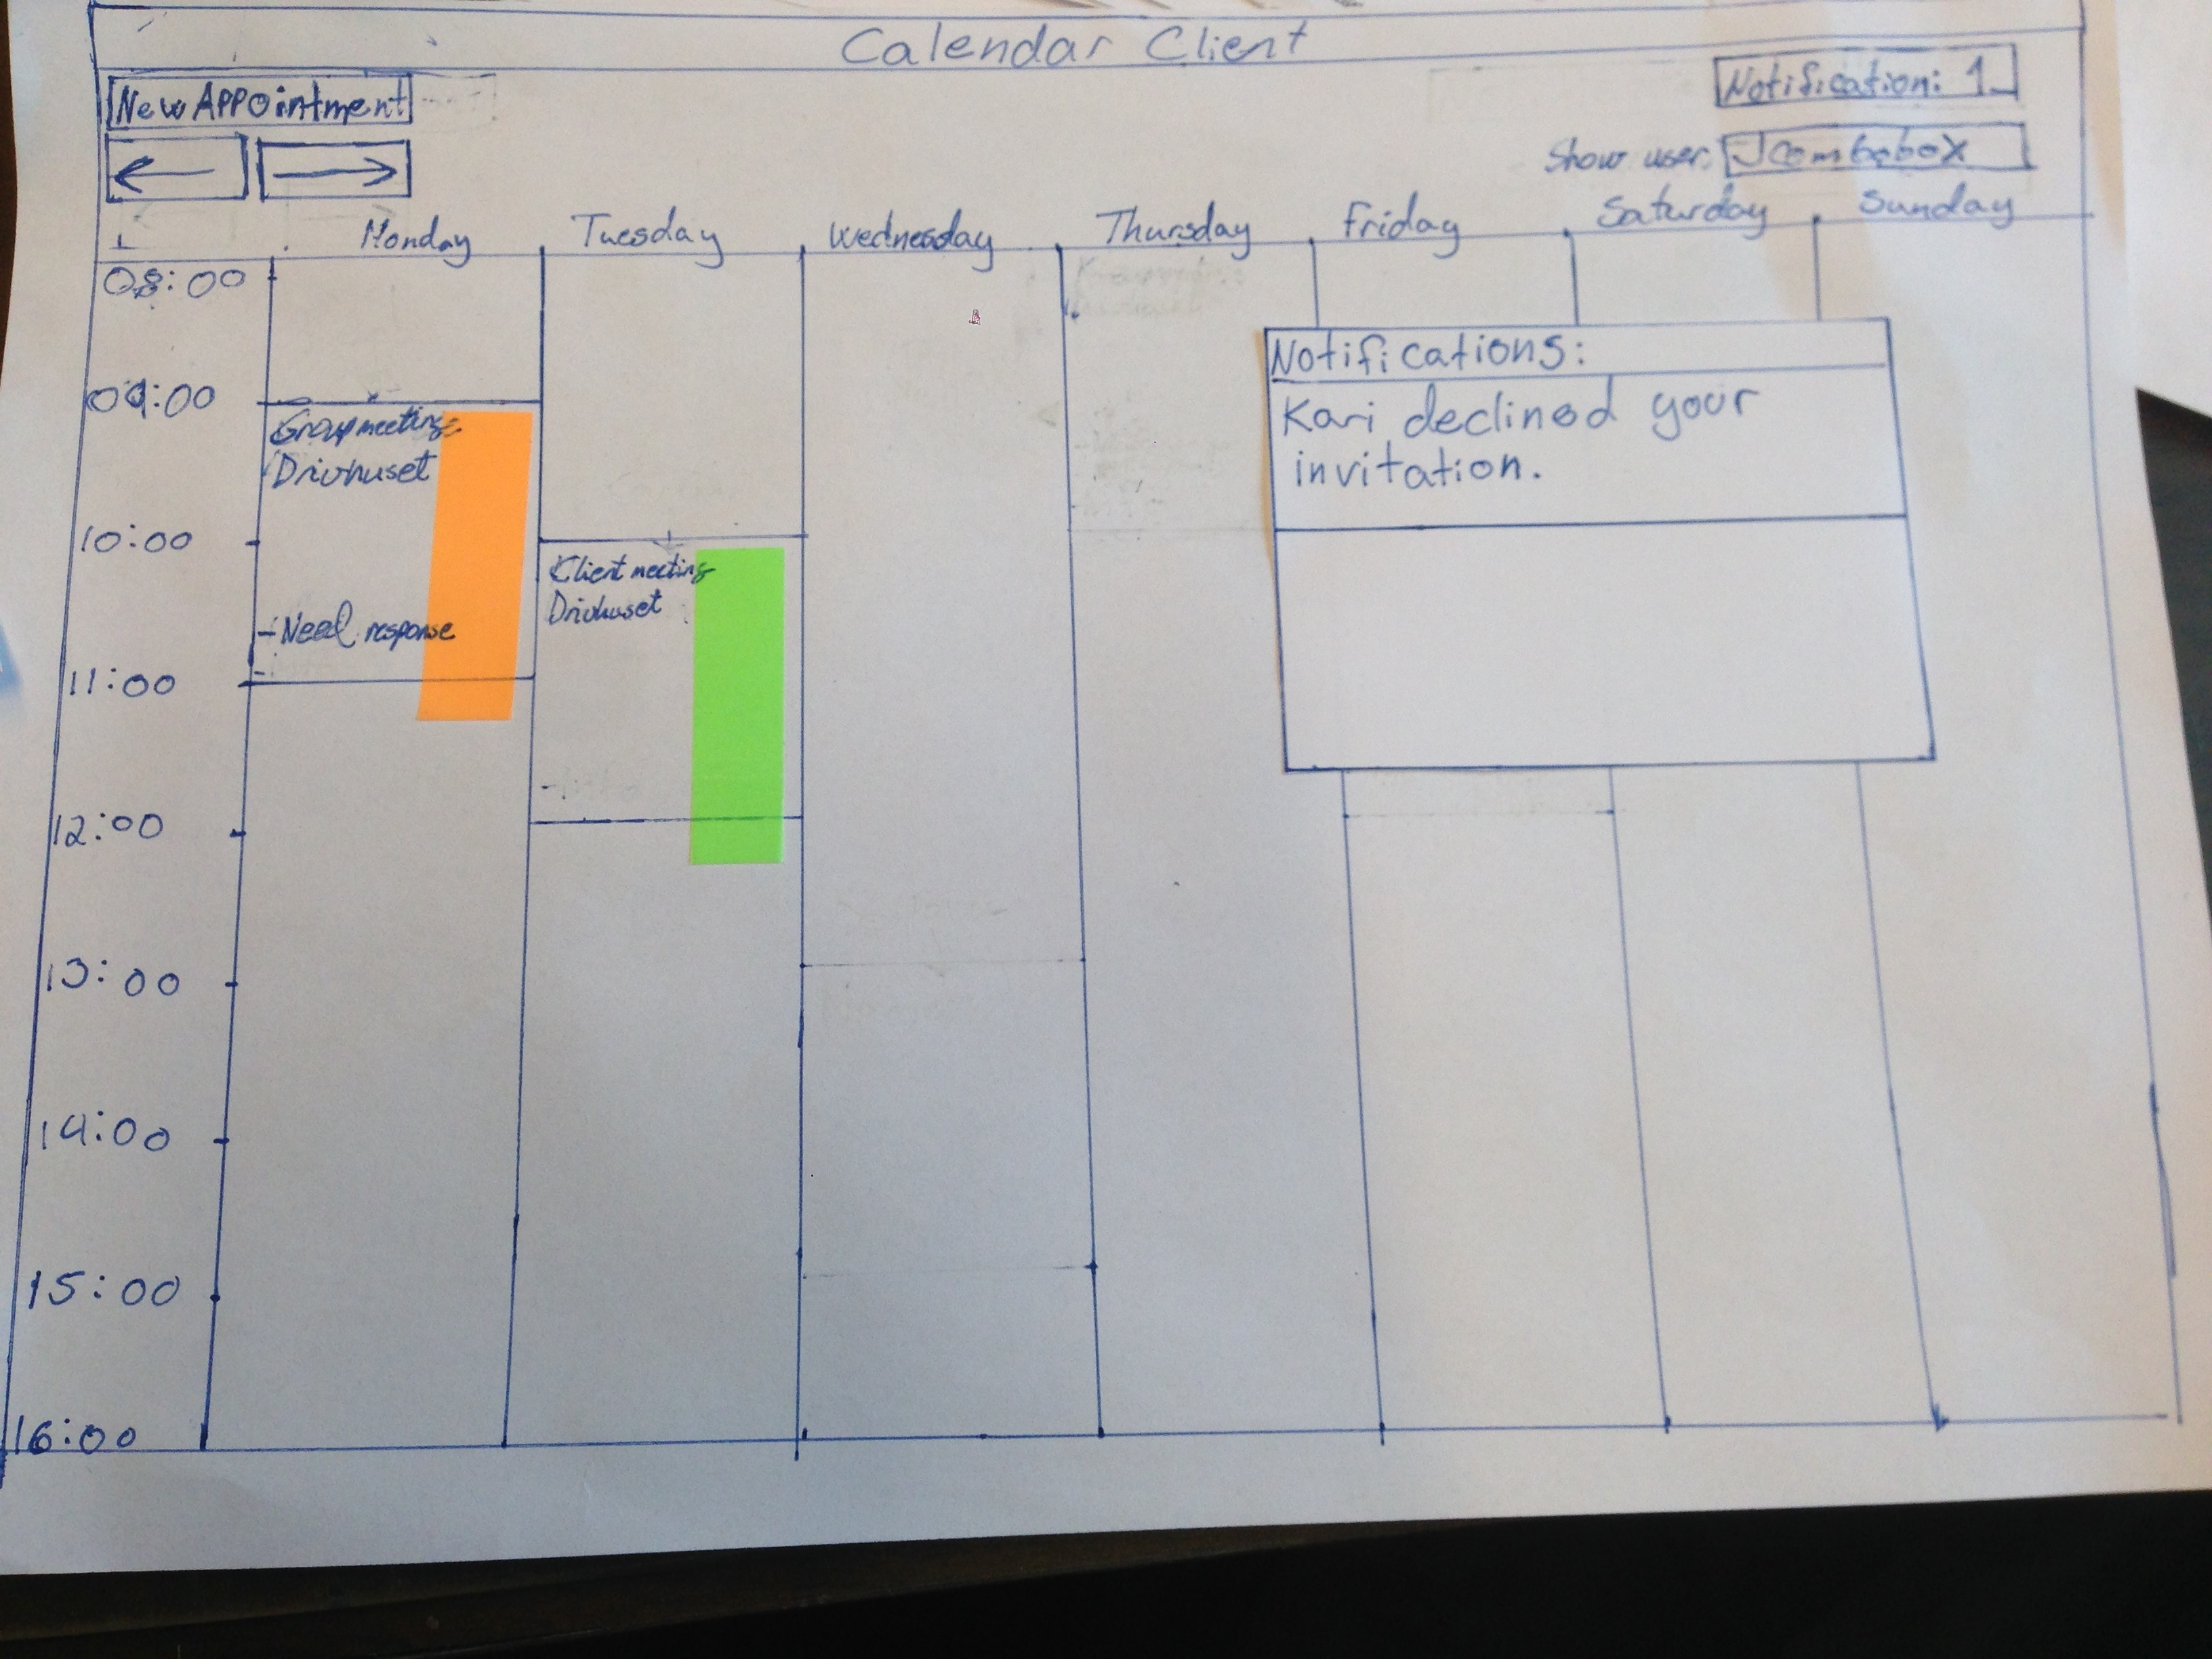
\includegraphics[width=8cm]{img/IMG_5608.JPG}
        \caption{Notification popup}
    \label{notificationpopup}
    \end{center}
\end{figure}

This is the notification popup screen. From here the users notifications will be listed. By clicking them, the user will be shown the view of the clicked appoiontment.

\newpage


\begin{figure}[h!] 
    \begin{center} 
        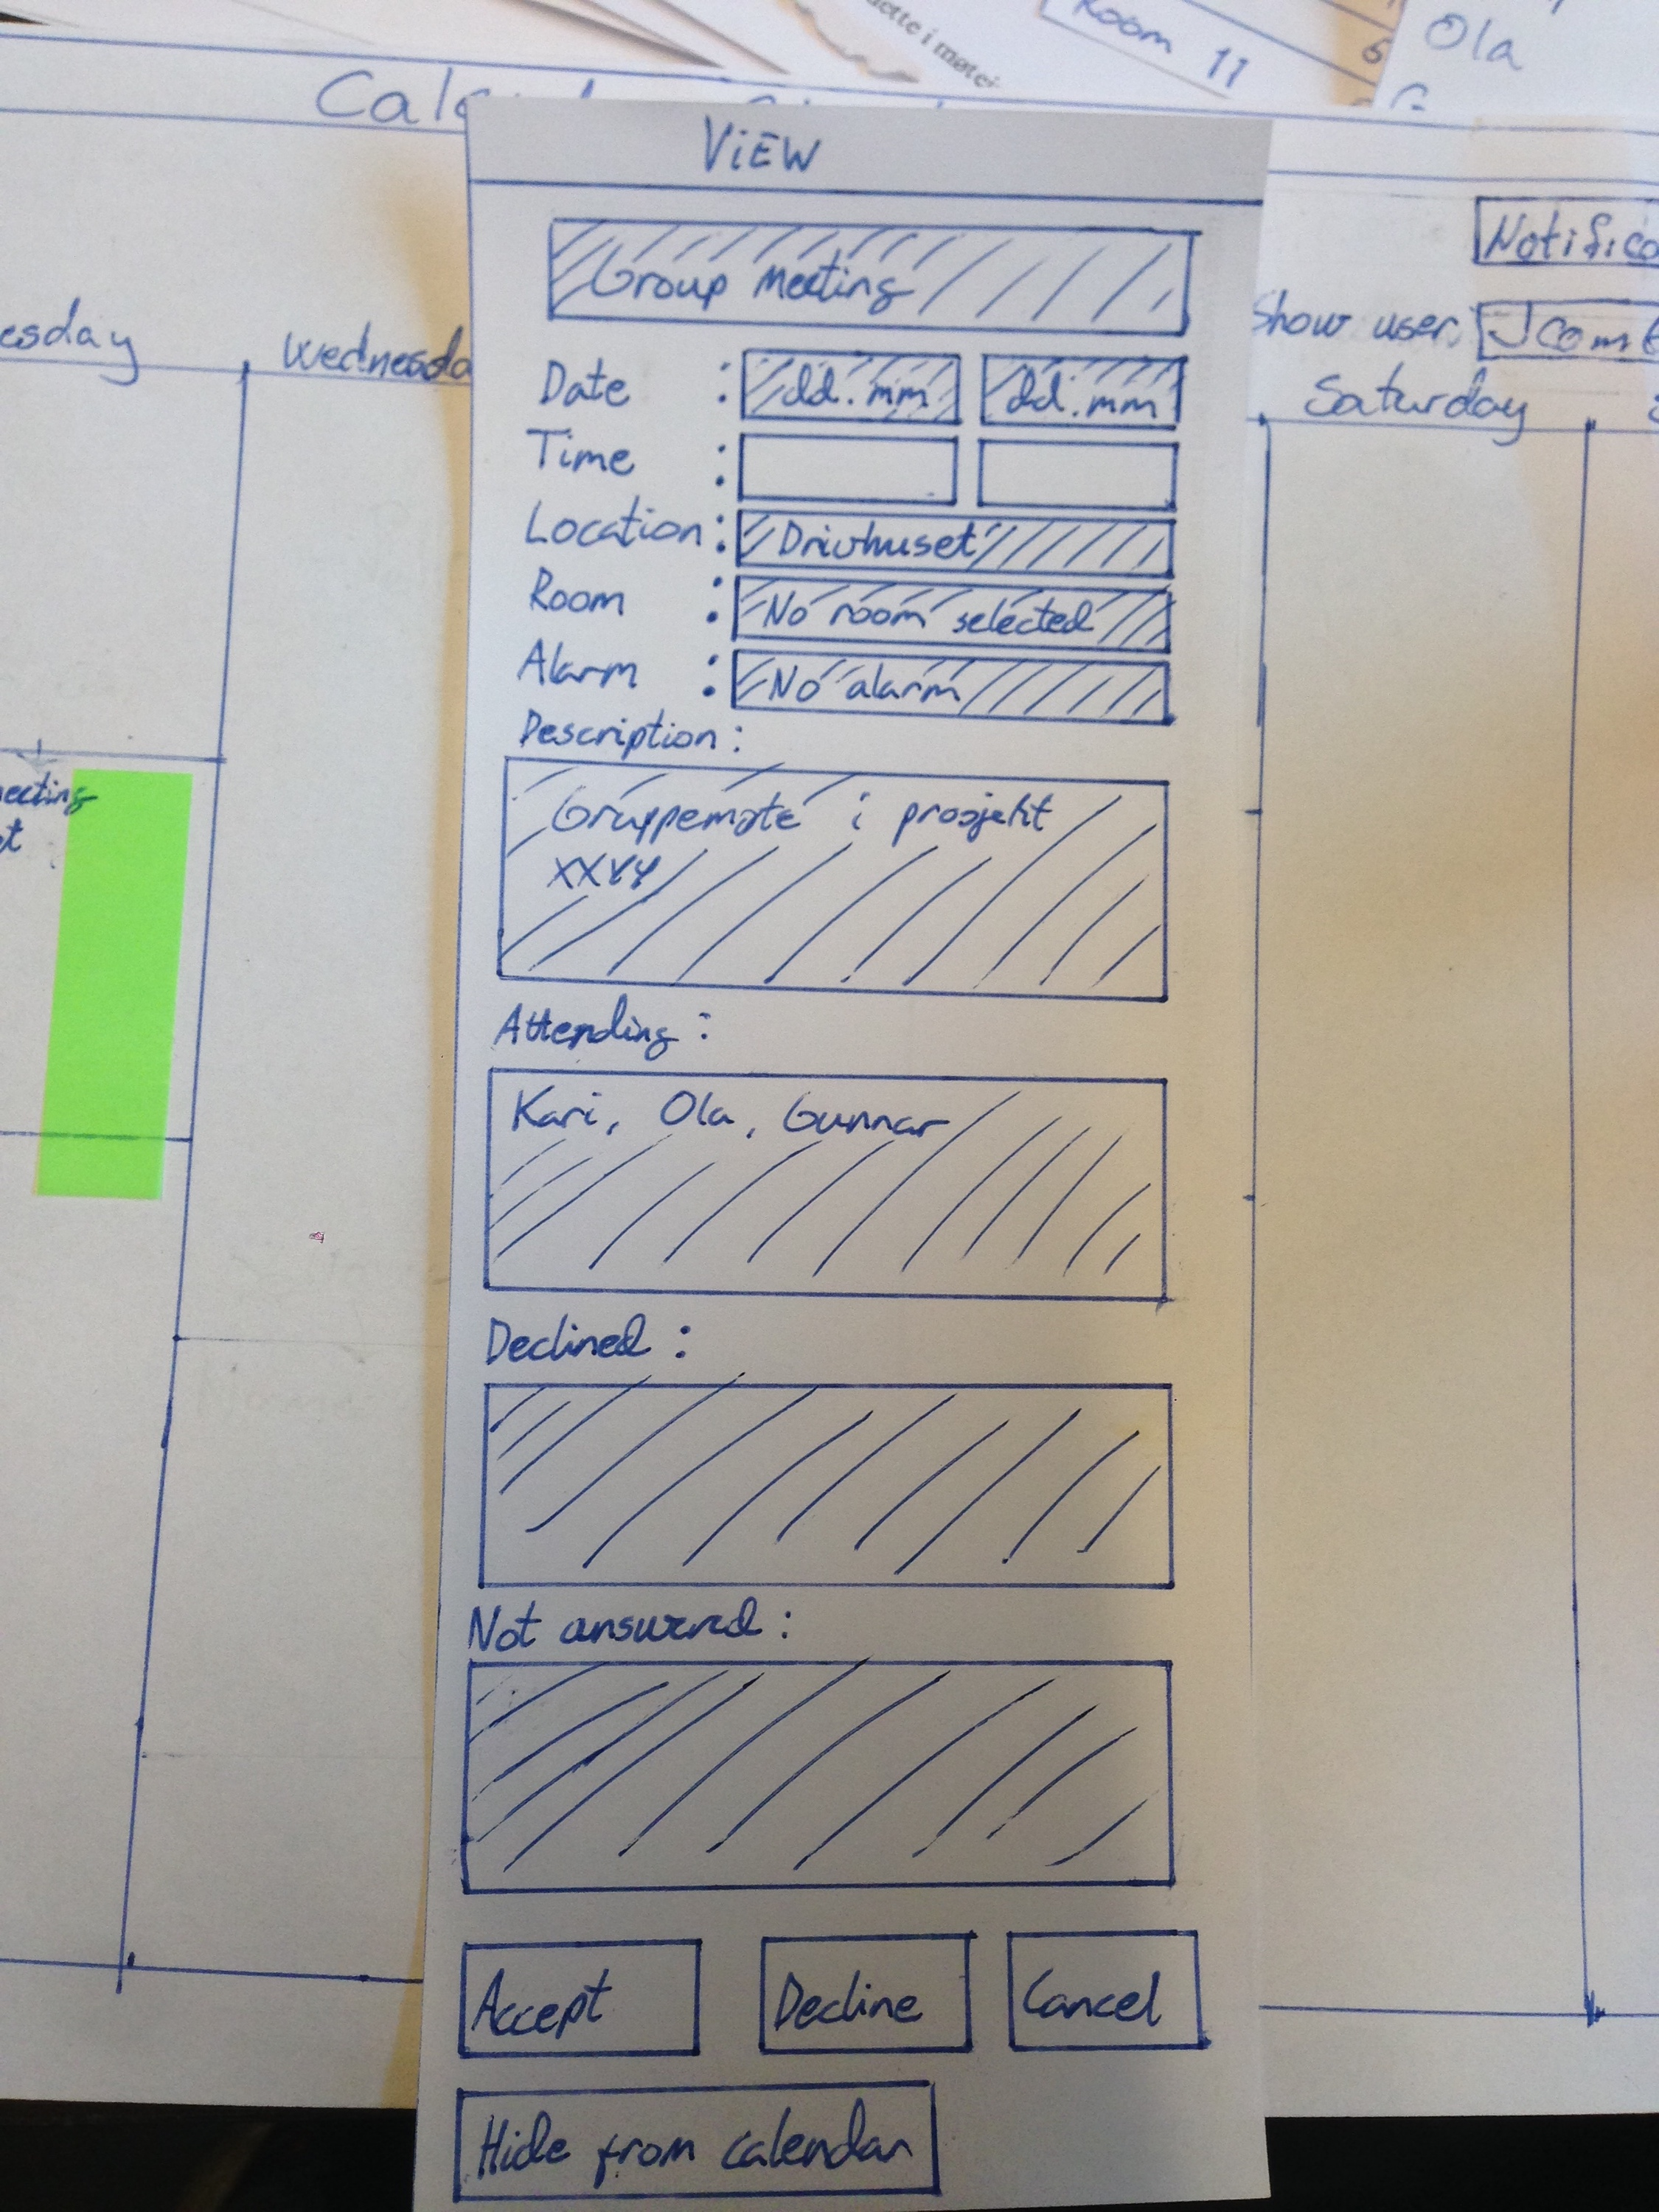
\includegraphics[width=8cm]{img/IMG_5609.JPG}
        \caption{Appointment view}
    \label{appointmentview}
    \end{center}
\end{figure}

When a user views an appointment, this is the screen presented. The marked out fields are non editable. The user can here press "accept" to accept the appointment, or press decline if the user is busy at the specified time for the meeting. By pressing "cancel", he will close the window without making any changes, and by pressing "Hide from calendar"-button, the appointment will be removed from this users calendar.

\newpage

\begin{figure}[h!] 
    \begin{center} 
        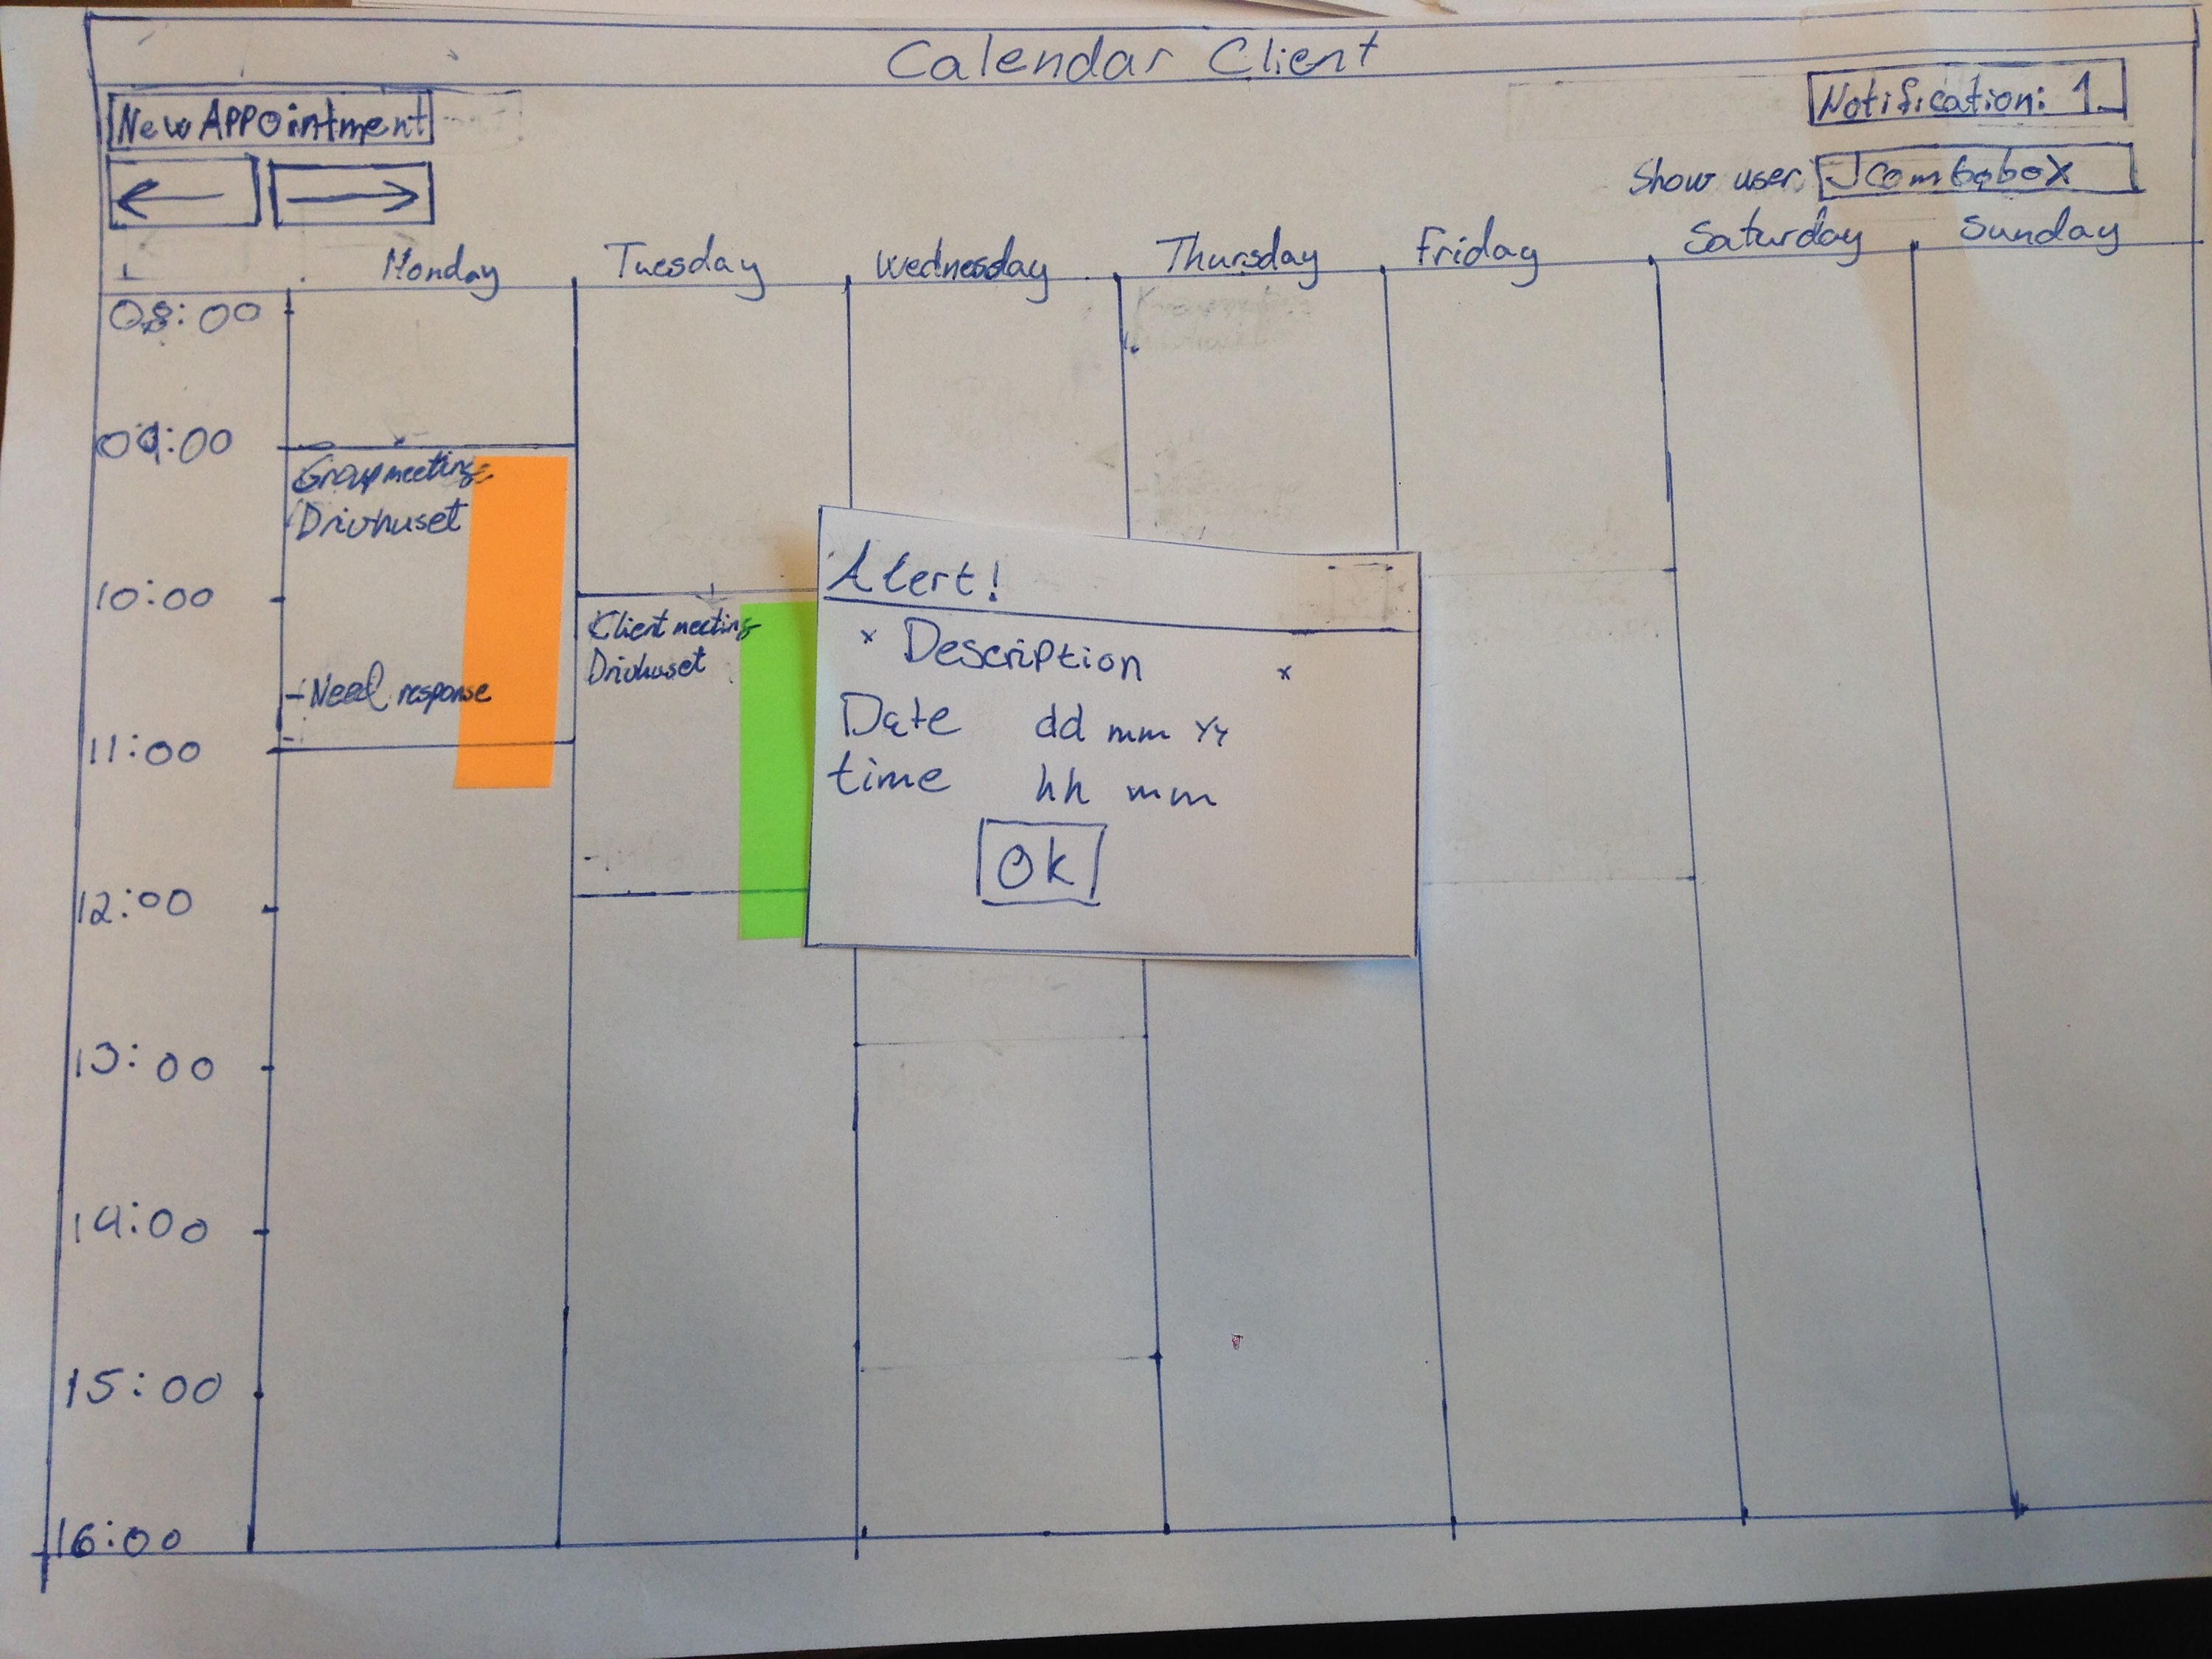
\includegraphics[width=8cm]{img/IMG_5611.JPG}
        \caption{Alert}
    \label{nalert}
    \end{center}
\end{figure}

This is an alert. It appears at the preset time, which the user chose when he viewed/made the appointment. By pressing "OK", the window closes.

\newpage



\section{The task at hand}
A usability test was performed to test the paperprototype. The tasks was as follows:
\begin{enumerate}

\item You shall invite a business connection to a meeting in your companys own meetingrooms (already registered in the system). You will invite Kari to a meeting from 12:00 - 14:00, 10. march, and you're supposed to book a meeting room through this calendar system.

\item Kari has now received a phonecall. Unfortunately she have to go to another more imortant meeting at the time you invited her. You will now be Kari and decline the appointment you were invited to first.

\item You're yourself again, and you have received a notification. Check this.

\item Delete Kari from this meeting and and Sindre instead.

\item Yor businessconnection calls you, and tell you he's one hour late. Change this in the appointment in the calendar.
\end{enumerate}


\section{The test}
\subsection{With student assistant}
\subsubsection*{Roles}
\begin{itemize}
\item Testleader: Jonas André Dalseth and Andreas Wien
\item Observers: Jonas André Dalseth, Finn Inderby, Espen Albert
\item Wizard Of Oz: Jonas André Dalseth og Andreas Wien
\item Tester: Fredrik Winther Dahl
\end{itemize}

\subsubsection*{Exectution}
The test with the student assistant wasn't very organized. First we thought we was just supposed to show him the paper model, so we didn't have any routines. Everybody on the group guided him through different scenarios, and we hadn't made any before we met him. After the test we asked him to fill out the SUS scheme and asked him what he thought about the system. We learned a lot about talking to him, and he told us how we should do it when we tested with the other group. 


\subsection{With other group}
\subsubsection*{Roles}
\begin{itemize}
\item Testleader: Jonas André Dalseth
\item Wizard of Oz: Andreas Wien
\item Observers: Finn Inderhaug, Kristoffer Dalby
\item Tester: Ole Halvor Dahl
\end{itemize}

\subsubsection*{Execution}
We met another group also working with the common project. The other group had chosen one person who would test our system. We chose one test leader, one "wizard of oz" and two people who wrote down the results from the test. The testleader presented how the test will work, what we are testing and how we are gonna do it. The test started, and the tester did the task presented above, without help from anyone of us. When the test was finished, he filled in a SUS diagram, and we asked him what he thought about the system.

\section{Results}
\subsection{With student assistant}
Our student assistant gave us a lot of valued response on both how we executed the test and how our system worked. The changes suggested to our execution were extremely helpful before our second testgroup, and included the following:
\begin{enumerate}
\item Select a test leader and a person to serve as your system.
\item Test leader should introduce the test, pointing out that it's the system that's being tested. 
\item Test subject should be given a set of scenarios or tasks to properly test the system. 
\item Test subject should be informed that (s)he may abort the test at any time.
\item Test subject should not be assisted in any way once the test starts.
\item Only the test leader should hold a dialog with the test subject.
\item The remaining members should be observing and noting any difficulties occuring during the test.
\end{enumerate}

The suggestions for the paper prototype included the following points:
\begin{enumerate}
\item The notifications popup was a bit difficult to understand because of a lack of division between elements in the list.
\item There was no support for clicking at a desired time and date directly in the calendar to create a new appointment.
\item When editing or creating an appointment the list of meeting rooms didn't show how many participants a room could hold.
\item When editing or creating an appointment it's not intuitive how to add more members.
\end{enumerate}

\subsection{With other group}
\begin{enumerate}
\item The test subject could not find the dates for the weekdays in the calendar view.
\end{enumerate}

\section{Redesign}
\begin{enumerate}
\item Make it possible for one notification to take more space than one line, and make them more separated.
\item This is a extra feature, so we will only implement it if we get time to do it
\item Make a add all alternative in JComboBox
\item The view will be changed so the size of the room will appear in the JComboBox, such that it appears next to the name om the meeting room
\item Show dates next to the days in the calendar


\end{document}